\documentclass[10pt,a4paper,oneside]{article}
\usepackage{cmap}
\usepackage[T2A]{fontenc}
\usepackage{float}
\usepackage{listings}
\usepackage{csquotes}
\usepackage[utf8]{inputenc}
\usepackage{amsmath}
\usepackage{amsfonts}
\usepackage{amssymb}
\usepackage[english, russian]{babel}%Подключаем русский язык.
\usepackage{graphicx}
\usepackage{geometry} % Меняем поля страницы.
\geometry{left=3cm} %Левое поле.
\geometry{right=2cm} %Правое поле.
\geometry{top=3cm} %Верхнее поле.
\geometry{bottom=2cm} %Нижнее поле.


%Начало документа
\begin{document}

%Создаём титульник.
\begin{titlepage}
\newpage
	%Название ВУЗа и институт.
	\begin{center}
		\Large Санкт-Петербургский Государственный Политехнический Университет\\
		Институт Компьютерных Наук и Технологий\\
	\end{center}
	%Кафедра.
	\begin{center}
		\large\textbf {Высшая школа интеллектуальных систем и суперкомпьютерных технологий}
	\end{center}
	
	%Пропуск места. 
	\vspace{5em}
	%!!!!!!!!!!!!!!!!!!!!!!!!!!!!!!!!!Название работы.
	\begin{center}
		\large{Отчёт по лабораторной работе №11 \\ на тему \\
		\textbf{Модуляция и выборка} }
	\end{center}
	
	%Делаем пропуск и пишем студента и преподавателя.
	\vspace{25em}
	\begin{flushright}
		\textbf{Работу выполнил\\}Студент группы 3530901/80203 \\ Танашкин В.А.\\
		\textbf{Преподаватель\\}Богач Н.В. 
	\end{flushright}
	
	\vspace{\fill}%В самом низу
	\begin{center}
	Санкт-Петербург, 2021 год	
	\end{center}
\end{titlepage} %Закончили титульный лист.

\section{Настройка проекта}
Перед тем как выполнять задания необходимо настроить проект и сделать все необходимые импорты:

\begin{figure}[H]
        \centering
        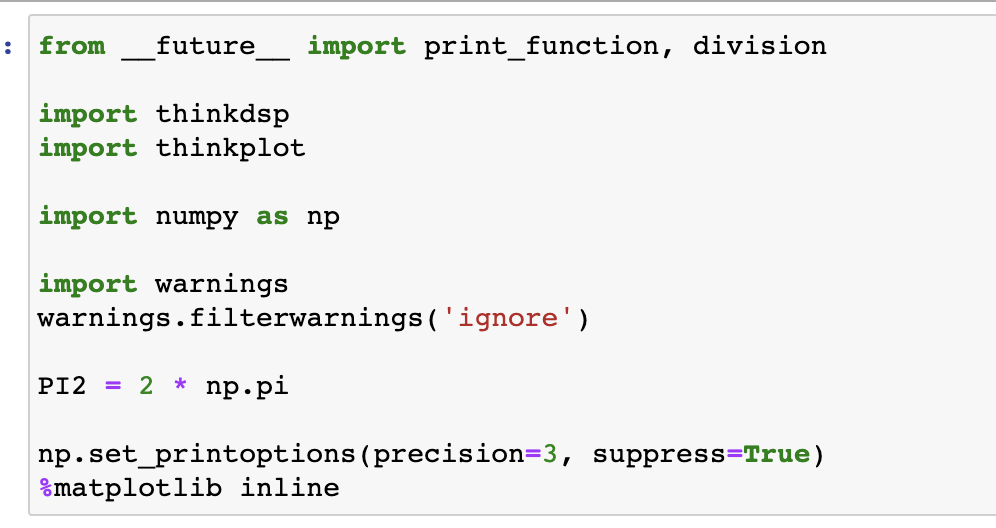
\includegraphics[width=0.75\textwidth]{pics/0.png}
        \caption{2}
        \label{fig:first}
\end{figure}

\section{Ход работы:}

Возьмем звук из репозитория:

\begin{figure}[H]
        \centering
        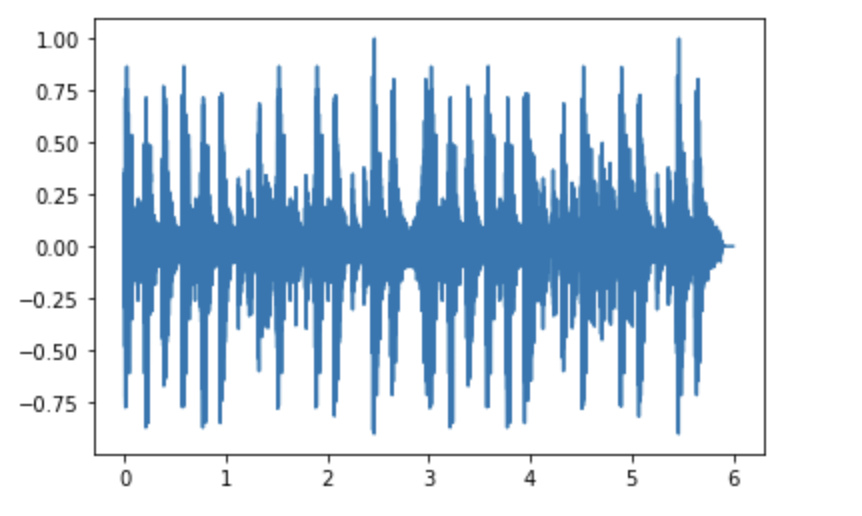
\includegraphics[width=0.75\textwidth]{pics/1.png}
        \caption{2}
        \label{fig:first}
\end{figure}

Этот сигнал дискретизируется с частотой 44100 Гц. Распечатаем спектр

\begin{figure}[H]
        \centering
        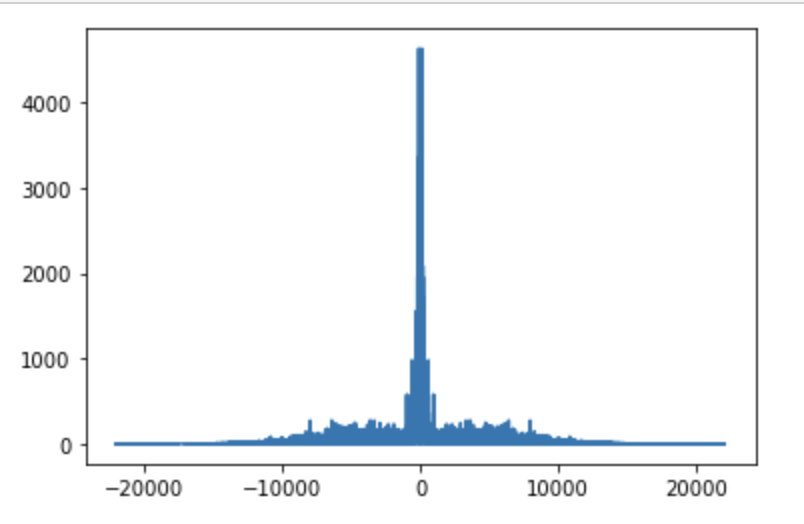
\includegraphics[width=0.75\textwidth]{pics/2.png}
        \caption{2}
        \label{fig:first}
\end{figure}

Уменьшим частоту дискретизации в 3 раза:

Перед дискретизацией мы применяем фильтр сглаживания, чтобы удалить частоты выше новой частоты свертки, которая равна частоте кадров / 2:

\begin{figure}[H]
        \centering
        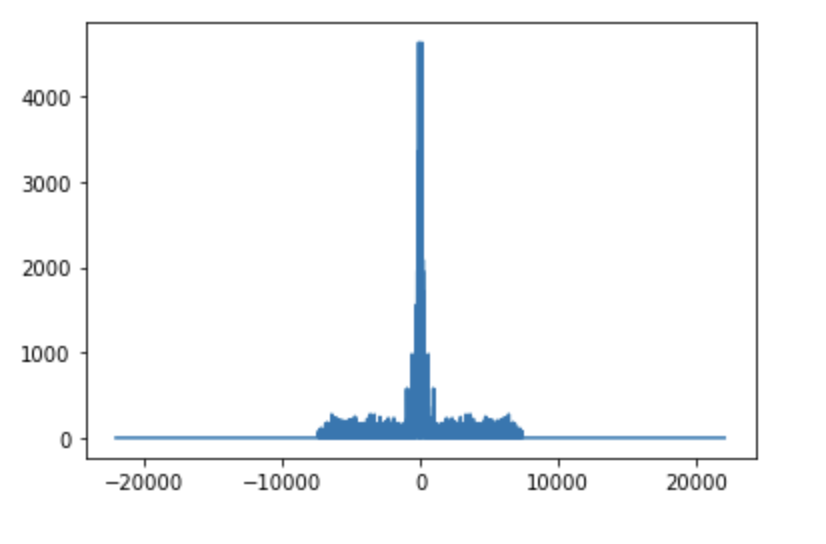
\includegraphics[width=0.75\textwidth]{pics/3.png}
        \caption{2}
        \label{fig:first}
\end{figure}

Реализуем функцию, которая имитирует процесс выборки:

\begin{figure}[H]
        \centering
        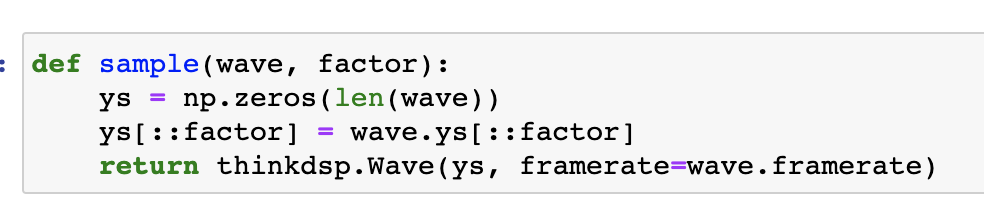
\includegraphics[width=0.75\textwidth]{pics/4.png}
        \caption{2}
        \label{fig:first}
\end{figure}

Результат содержит копии спектра около 20 кГц, но они практически незаметны на слух, но мы сможем их рассмотреть на спектре:

\begin{figure}[H]
        \centering
        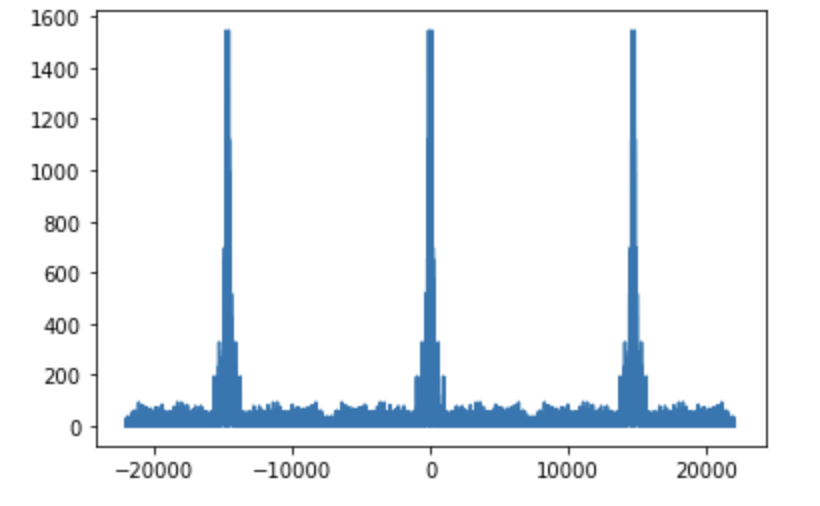
\includegraphics[width=0.75\textwidth]{pics/5.png}
        \caption{2}
        \label{fig:first}
\end{figure}

Мы можем избавиться от спектральных копий, снова применив фильтр сглаживания:

\begin{figure}[H]
        \centering
        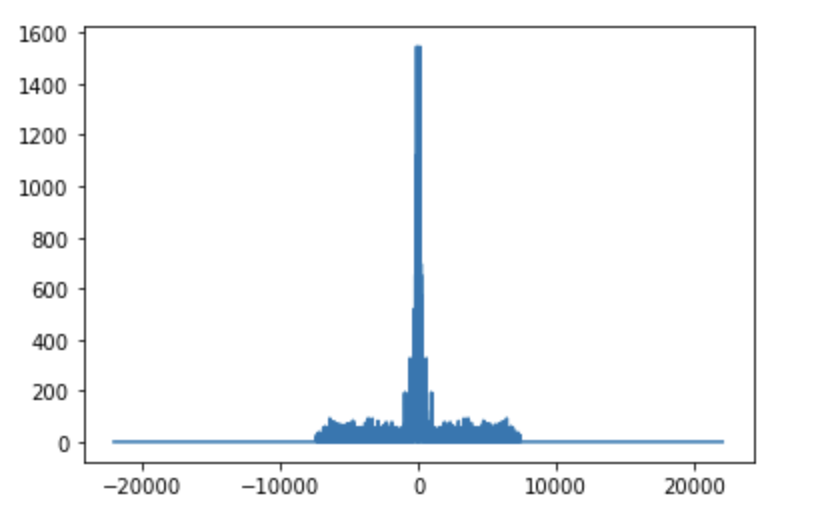
\includegraphics[width=0.75\textwidth]{pics/6.png}
        \caption{2}
        \label{fig:first}
\end{figure}

Мы только что потеряли половину энергии в спектре, но мы можем масштабировать результат, чтобы вернуть его:

\begin{figure}[H]
        \centering
        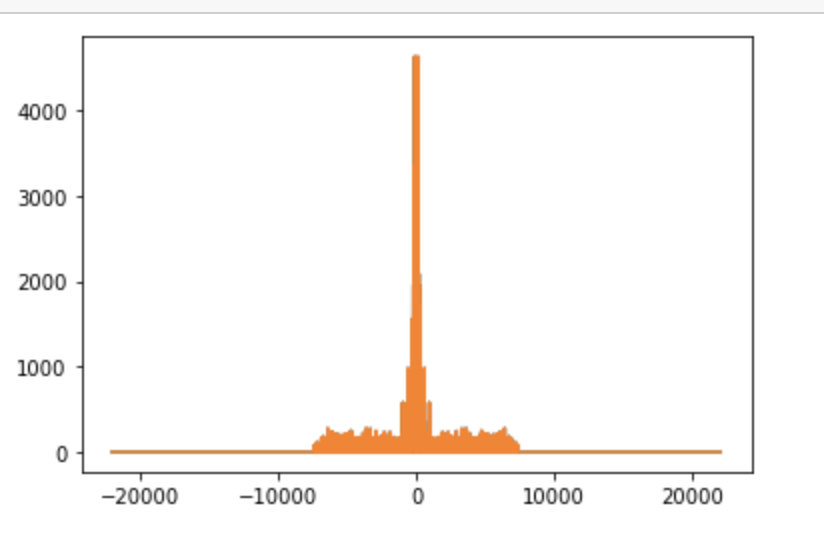
\includegraphics[width=0.75\textwidth]{pics/7.png}
        \caption{2}
        \label{fig:first}
\end{figure}

Теперь разница между спектром до и после дискретизации должна быть небольшой.

\begin{figure}[H]
        \centering
        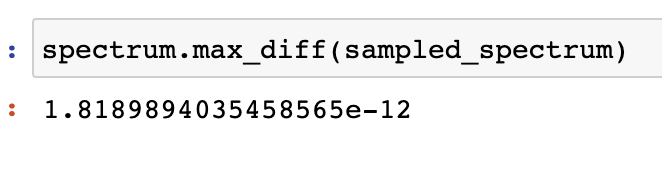
\includegraphics[width=0.75\textwidth]{pics/8.png}
        \caption{2}
        \label{fig:first}
\end{figure}

Преобразуем обратно в волну, разница между интерполированной волной и фильтрованной волной также должна быть небольшой.

\begin{figure}[H]
        \centering
        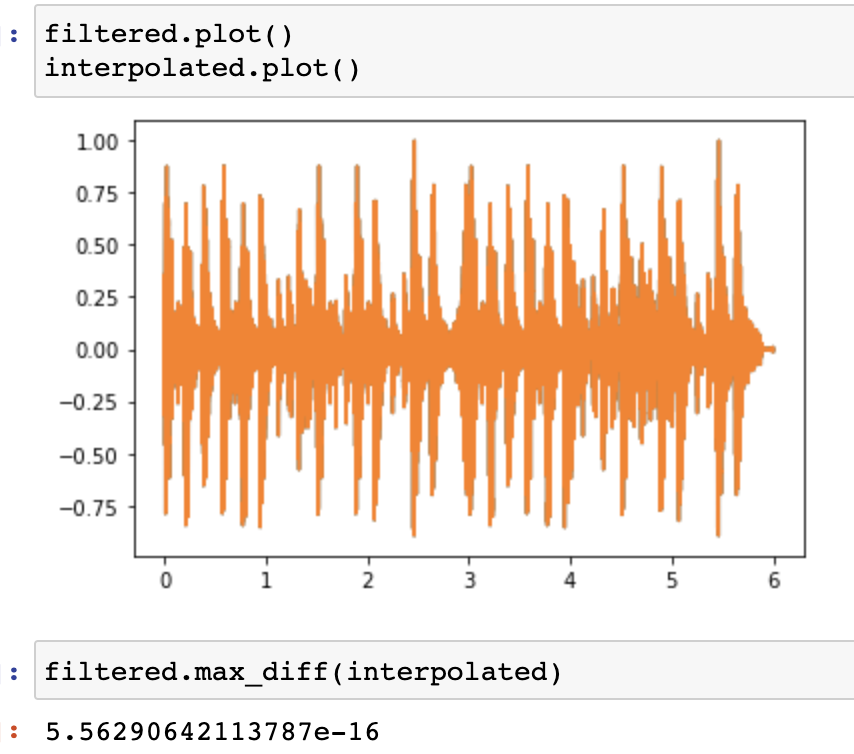
\includegraphics[width=0.75\textwidth]{pics/9.png}
        \caption{2}
        \label{fig:first}
\end{figure}

\end{document}
